\documentclass[]{article}
\usepackage{lmodern}
\usepackage{amssymb,amsmath}
\usepackage{ifxetex,ifluatex}
\usepackage{fixltx2e} % provides \textsubscript
\ifnum 0\ifxetex 1\fi\ifluatex 1\fi=0 % if pdftex
  \usepackage[T1]{fontenc}
  \usepackage[utf8]{inputenc}
\else % if luatex or xelatex
  \ifxetex
    \usepackage{mathspec}
  \else
    \usepackage{fontspec}
  \fi
  \defaultfontfeatures{Ligatures=TeX,Scale=MatchLowercase}
\fi
% use upquote if available, for straight quotes in verbatim environments
\IfFileExists{upquote.sty}{\usepackage{upquote}}{}
% use microtype if available
\IfFileExists{microtype.sty}{%
\usepackage{microtype}
\UseMicrotypeSet[protrusion]{basicmath} % disable protrusion for tt fonts
}{}
\usepackage[margin=1in]{geometry}
\usepackage{hyperref}
\hypersetup{unicode=true,
            pdftitle={Waldman triage},
            pdfauthor={DJM},
            pdfborder={0 0 0},
            breaklinks=true}
\urlstyle{same}  % don't use monospace font for urls
\usepackage{longtable,booktabs}
\usepackage{graphicx,grffile}
\makeatletter
\def\maxwidth{\ifdim\Gin@nat@width>\linewidth\linewidth\else\Gin@nat@width\fi}
\def\maxheight{\ifdim\Gin@nat@height>\textheight\textheight\else\Gin@nat@height\fi}
\makeatother
% Scale images if necessary, so that they will not overflow the page
% margins by default, and it is still possible to overwrite the defaults
% using explicit options in \includegraphics[width, height, ...]{}
\setkeys{Gin}{width=\maxwidth,height=\maxheight,keepaspectratio}
\IfFileExists{parskip.sty}{%
\usepackage{parskip}
}{% else
\setlength{\parindent}{0pt}
\setlength{\parskip}{6pt plus 2pt minus 1pt}
}
\setlength{\emergencystretch}{3em}  % prevent overfull lines
\providecommand{\tightlist}{%
  \setlength{\itemsep}{0pt}\setlength{\parskip}{0pt}}
\setcounter{secnumdepth}{5}
% Redefines (sub)paragraphs to behave more like sections
\ifx\paragraph\undefined\else
\let\oldparagraph\paragraph
\renewcommand{\paragraph}[1]{\oldparagraph{#1}\mbox{}}
\fi
\ifx\subparagraph\undefined\else
\let\oldsubparagraph\subparagraph
\renewcommand{\subparagraph}[1]{\oldsubparagraph{#1}\mbox{}}
\fi

%%% Use protect on footnotes to avoid problems with footnotes in titles
\let\rmarkdownfootnote\footnote%
\def\footnote{\protect\rmarkdownfootnote}

%%% Change title format to be more compact
\usepackage{titling}

% Create subtitle command for use in maketitle
\newcommand{\subtitle}[1]{
  \posttitle{
    \begin{center}\large#1\end{center}
    }
}

\setlength{\droptitle}{-2em}

  \title{Waldman triage}
    \pretitle{\vspace{\droptitle}\centering\huge}
  \posttitle{\par}
    \author{DJM}
    \preauthor{\centering\large\emph}
  \postauthor{\par}
      \predate{\centering\large\emph}
  \postdate{\par}
    \date{June 6, 2016}


\begin{document}
\maketitle

Outline: see waldman-suggestions

In order of decreasing priority (balancing ease of implementation
against impact):

\begin{enumerate}
\item Suggestion 3.4: check whether the best permuted models swap hours worked
  for ``another flow variable''.
\item Suggestion 2.2: pick some of the best permutations and plot their
  predictions along with those of the baseline, un-permuted model.
\item Suggestion 3.3: a detailed examination of the best permuted model.
\item Suggestion 1.4: do the ``deep'' parameters co-vary with the policy parameters?
\item Suggestion 1.3: look at out-of-sample forecasts under a different policy
  rule.
\item Suggestion 3.1: $p$-value for how much the SW model is beaten by its
  permutations.
\end{enumerate}

\hypertarget{does-the-best-permuted-model-swap-hours-worked}{%
\section{Does the best (permuted) model swap hours
worked?}\label{does-the-best-permuted-model-swap-hours-worked}}

\begin{longtable}[]{@{}lllllll@{}}
\caption{Top 20 permutations based on (penalized) log-likelihood. The
top row is the correct ordering. Hours worked should be in the first
column.}\tabularnewline
\toprule
labobs & robs & pinfobs & dy & dc & dinve & dw\tabularnewline
\midrule
\endfirsthead
\toprule
labobs & robs & pinfobs & dy & dc & dinve & dw\tabularnewline
\midrule
\endhead
labobs & pinfobs & robs & dy & dw & dc & dinve\tabularnewline
labobs & robs & pinfobs & dc & dw & dy & dinve\tabularnewline
labobs & robs & pinfobs & dy & dw & dinve & dc\tabularnewline
pinfobs & labobs & robs & dy & dc & dw & dinve\tabularnewline
pinfobs & robs & labobs & dy & dw & dinve & dc\tabularnewline
pinfobs & robs & labobs & dc & dw & dy & dinve\tabularnewline
pinfobs & robs & labobs & dy & dc & dinve & dw\tabularnewline
labobs & robs & pinfobs & dw & dy & dinve & dc\tabularnewline
labobs & robs & pinfobs & dinve & dy & dw & dc\tabularnewline
pinfobs & robs & labobs & dc & dinve & dy & dw\tabularnewline
robs & pinfobs & labobs & dinve & dc & dy & dw\tabularnewline
robs & pinfobs & labobs & dy & dc & dinve & dw\tabularnewline
robs & pinfobs & labobs & dc & dw & dy & dinve\tabularnewline
labobs & robs & pinfobs & dw & dc & dy & dinve\tabularnewline
robs & labobs & pinfobs & dc & dy & dinve & dw\tabularnewline
labobs & robs & pinfobs & dw & dinve & dy & dc\tabularnewline
pinfobs & robs & labobs & dw & dy & dinve & dc\tabularnewline
labobs & pinfobs & robs & dw & dy & dinve & dc\tabularnewline
pinfobs & robs & labobs & dy & dw & dc & dinve\tabularnewline
labobs & pinfobs & robs & dc & dy & dinve & dw\tabularnewline
\bottomrule
\end{longtable}

\hypertarget{plot-some-predictions-along-with-the-best-model}{%
\section{Plot some predictions along with the best
model}\label{plot-some-predictions-along-with-the-best-model}}

The following plots show the top 20 flips based on ``average percent
improvement'' (this is a post-hoc measure). Blue-dotted is observed data
while red is the SW model.

\begin{center}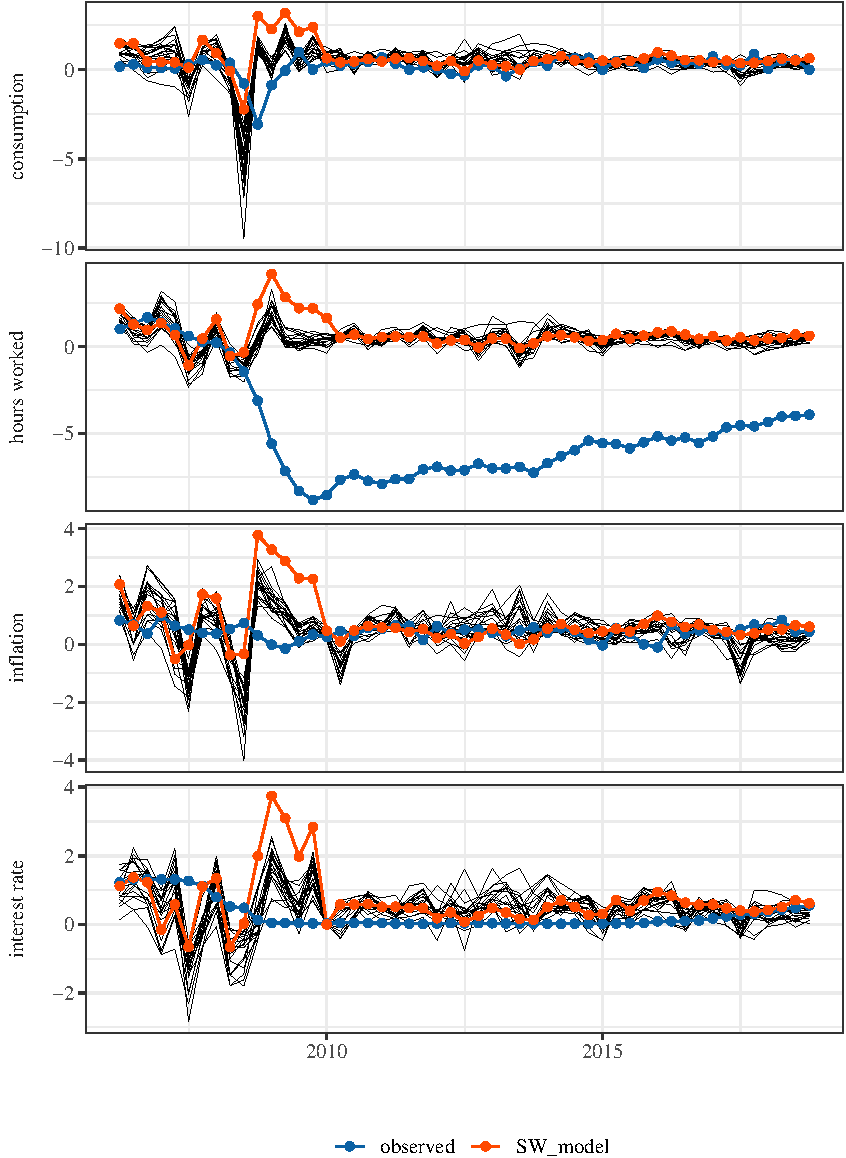
\includegraphics{waldman-triage_files/figure-latex/pc-preds-p1-1} \end{center}

\begin{center}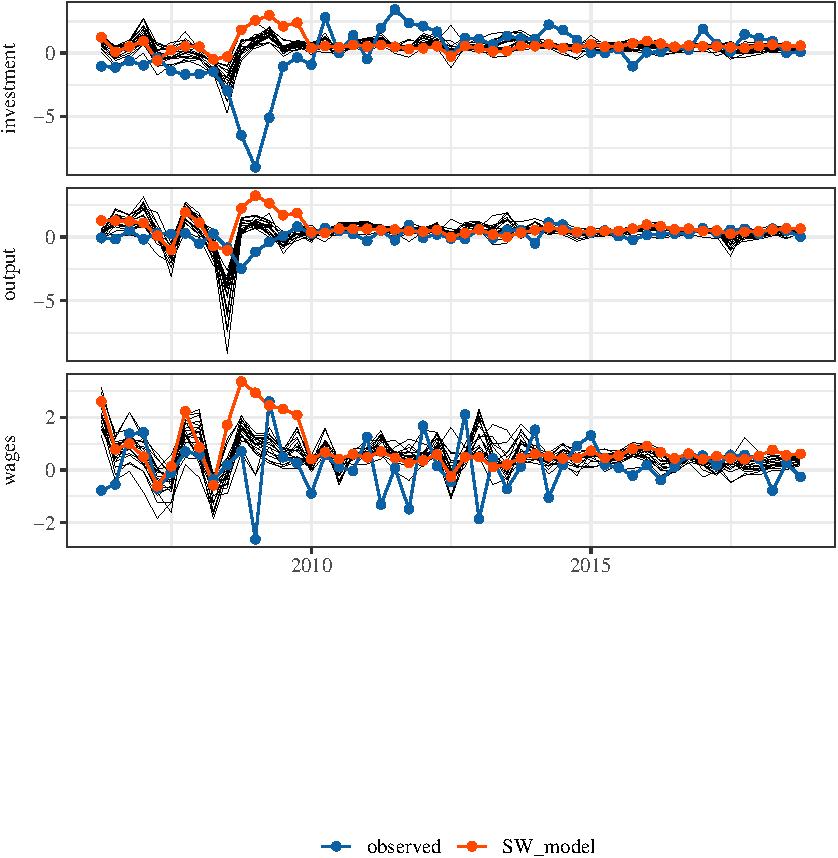
\includegraphics{waldman-triage_files/figure-latex/pc-preds-p2-1} \end{center}

\clearpage

The next set of plots is the Top 20 permutations by negative (penalized)
log-likelihood.

\begin{center}\includegraphics{waldman-triage_files/figure-latex/llike-preds-p1-1} \end{center}

\begin{center}\includegraphics{waldman-triage_files/figure-latex/llike-preds-p2-1} \end{center}

\clearpage

\hypertarget{best-model-by-penalized-log-likelihood}{%
\section{Best model by penalized
log-likelihood}\label{best-model-by-penalized-log-likelihood}}

The true model is

labobs, robs, pinfobs, dy, dc, dinve, dw

while the best one is

labobs, pinfobs, robs, dy, dw, dc, dinve.

This model is pretty clearly scary to a macroeconomist. First of all,
the standard model says that the monetary authority sets the interest
rate based on inflation and deviation of output from trend. This model
reverses cause and effect: inflation is the control variable while the
interest rate is the input to the Taylor rule. I think, actually, the
most interesting exercise would be to copy and paste the first section
of the SW paper, but change out all the notation.

I think it's also important to note here, that the penalized negative
log-likelihood is very flat relative to permutations. In terms of that
metric, 6.2\% of permutations are within 10\% of the true permutation.

\hypertarget{do-the-deep-parameters-co-vary-with-the-policy-parameters}{%
\section{Do the `deep' parameters co-vary with the policy
parameters?}\label{do-the-deep-parameters-co-vary-with-the-policy-parameters}}

\begin{longtable}[]{@{}lrrrr@{}}
\caption{Correlations between `deep' parameters and Taylor rule
parameters. From the `Simulate and estimate' exercise.}\tabularnewline
\toprule
& r{[}pi{]} & rho & r{[}y{]} & r{[}Delta{]}{[}y{]}\tabularnewline
\midrule
\endfirsthead
\toprule
& r{[}pi{]} & rho & r{[}y{]} & r{[}Delta{]}{[}y{]}\tabularnewline
\midrule
\endhead
phi1 & 0.197 & 0.097 & -0.034 & 0.113\tabularnewline
sigma{[}c{]} & 0.061 & 0.257 & 0.169 & 0.017\tabularnewline
h & 0.326 & 0.076 & 0.016 & -0.343\tabularnewline
xi{[}w{]} & -0.055 & 0.427 & 0.020 & 0.082\tabularnewline
sigma{[}l{]} & 0.006 & 0.190 & 0.033 & -0.373\tabularnewline
xi{[}p{]} & -0.261 & 0.360 & 0.125 & 0.186\tabularnewline
iota{[}w{]} & 0.096 & 0.036 & 0.052 & 0.007\tabularnewline
iota{[}p{]} & 0.027 & 0.168 & -0.027 & 0.038\tabularnewline
Psi & 0.340 & 0.005 & 0.104 & 0.331\tabularnewline
Phi & 0.019 & 0.031 & 0.030 & 0.021\tabularnewline
r{[}pi{]} & 1.000 & 0.315 & 0.235 & -0.004\tabularnewline
rho & 0.315 & 1.000 & 0.324 & 0.122\tabularnewline
r{[}y{]} & 0.235 & 0.324 & 1.000 & -0.036\tabularnewline
r{[}Delta{]}{[}y{]} & -0.004 & 0.122 & -0.036 & 1.000\tabularnewline
bar(pi) & -0.037 & -0.048 & -0.077 & 0.008\tabularnewline
100(beta\^{}\{-1\} -1) & -0.037 & -0.184 & -0.143 &
-0.043\tabularnewline
bar(l) & 0.066 & 0.104 & 0.077 & -0.050\tabularnewline
bar(gamma) & 0.017 & 0.035 & 0.050 & -0.015\tabularnewline
rho{[}ga{]} & -0.234 & -0.146 & -0.005 & 0.007\tabularnewline
alpha & 0.179 & 0.108 & 0.162 & -0.039\tabularnewline
\bottomrule
\end{longtable}

\hypertarget{simulate-from-the-model-change-taylor-parameters-examine-forecasts}{%
\section{Simulate from the model, change Taylor parameters, examine
forecasts}\label{simulate-from-the-model-change-taylor-parameters-examine-forecasts}}

\begin{enumerate}
\def\labelenumi{\arabic{enumi})}
\setcounter{enumi}{2}
\tightlist
\item
  the point of micro foundations is that they are supposed to give good
  conditional forecasts conditional on a change in policy. I think in
  the simulate, estimate, test out of sample effort it would be
  interesting to simulate, estimate, change policy parameters and test.
  The problem with ad hoc reduced form models is supposed to be that
  they include parameters which are not deep and structural and the same
  for different policy regimes but which depend on the policy. Changing
  the policy rule is supposed to illustrate the advantage of DSGE
\end{enumerate}

\begin{quotation} {\em Potentially interesting.  Presumably the model we use to
    generate the new-policy trajectories would be SW.  How hard would this be
    to do for a few of the best permutations?}
\end{quotation}

I'm not sure I see the relevance of this one. He seems to suggest
simulating from the baseline many times, estimating on part of the time
series, then changing the parameters and forecasting the rest of the
time series (which was actually generated with different conditions). Is
the goal to determine if conditional forecasts are accurate? It seems
like we really want to do some sort of hypothesis test as follows:

\begin{enumerate}
\def\labelenumi{\arabic{enumi}.}
\tightlist
\item
  Generate data up to some change point \(T_1\). At the change point,
  alter only the policy parameters and generate the future from \(T_1\)
  to \(T_2\).
\item
  Estimate a model with a change point at \(T_1\). See whether allowing
  only the policy parameters to vary is sufficient, or if we need to let
  all the `deep' parameters vary.
\item
  Test the null that the policy parameters are enough (LRT).
\end{enumerate}

Considering that we're generating data out of, and then using, the
correct model, I find it hard to imagine we would reject the null (true)
model with a change point.

\hypertarget{p-value}{%
\section{P-value}\label{p-value}}

This is awful for the reasons previously discussed.

\hypertarget{another-one-3.2}{%
\section{Another one (3.2)}\label{another-one-3.2}}

or the other way, what if the permuted model with the highest penalized
likelihood were The Truth ? How badly would the SW model fit and
forecast ? Here I actually guess it would do OK.

\begin{quotation} {\em This seems easy, and gets at the but-are-the-permutations-really-different question.}
\end{quotation}

Procedure:

\begin{enumerate}
\def\labelenumi{\arabic{enumi}.}
\tightlist
\item
  generate data out of the best permutation.
\item
  get forecasts using it and the SW model (say 100 each). Which is
  better?
\end{enumerate}

The average negative log-likelihood of the true model is -1220 compared
to 409 for the SW model. The MSEs are 0.00389 compared to 0.00442
respectively. The next set of figures shows the data (black),
predictions from the true model (blue), and SW model (red).


\end{document}
